\documentclass[12pt,a4paper]{article}

\frenchspacing
\sloppy

\usepackage[utf8]{inputenc}
\usepackage{t1enc}
\usepackage[magyar]{babel}
\usepackage{hyperref}
\usepackage[dvipsnames]{xcolor}
\usepackage{listings}
\usepackage{graphicx}
\graphicspath{ {./img/} }
\lstset{
  language=C++,
  basicstyle={\small\ttfamily},
  keywordstyle=\color{blue},
  stringstyle=\color{red},
  backgroundcolor=\color{gray},
  commentstyle=\color{green}
}
\hypersetup{
    colorlinks=true,
    linkcolor=blue,
    filecolor=magenta,
    urlcolor=blue,
}
\urlstyle{same}

\title{Önálló laboratórium dokumentáció}
\author{Wágner Árpád (O2OFFX)}
\date{2019/20 - 2. félév}

\begin{document}
  \maketitle

  \section{Bevezetés}

    Ez a dokumentum tartalmazza az önálló laboratórium tárgy keretében elvégzett munkám dokumentációját.
    %TODO: Általános leírás arról, amit csináltunk

    A munka rám háruló része két felé osztható: az első részben feladatom volt egy bizonyos ESP32 lapka megismerése és lehetőségeinek felderítése. A második részben pedig egy, a későbbiekben diagnosztikai eszközként használandó mikrofonnal foglalkoztam.

    \textbf{Megjegyzés:} A laboratórium során létrejött forráskódok \href{https://github.com/awrpad/Onlab}{ezen}\footnote{A repository URL-je: \url{https://github.com/awrpad/Onlab}} a GitHub repository-n elérhetőek.

  \newpage

  \section{``Nagykijelzős'' ESP32}
    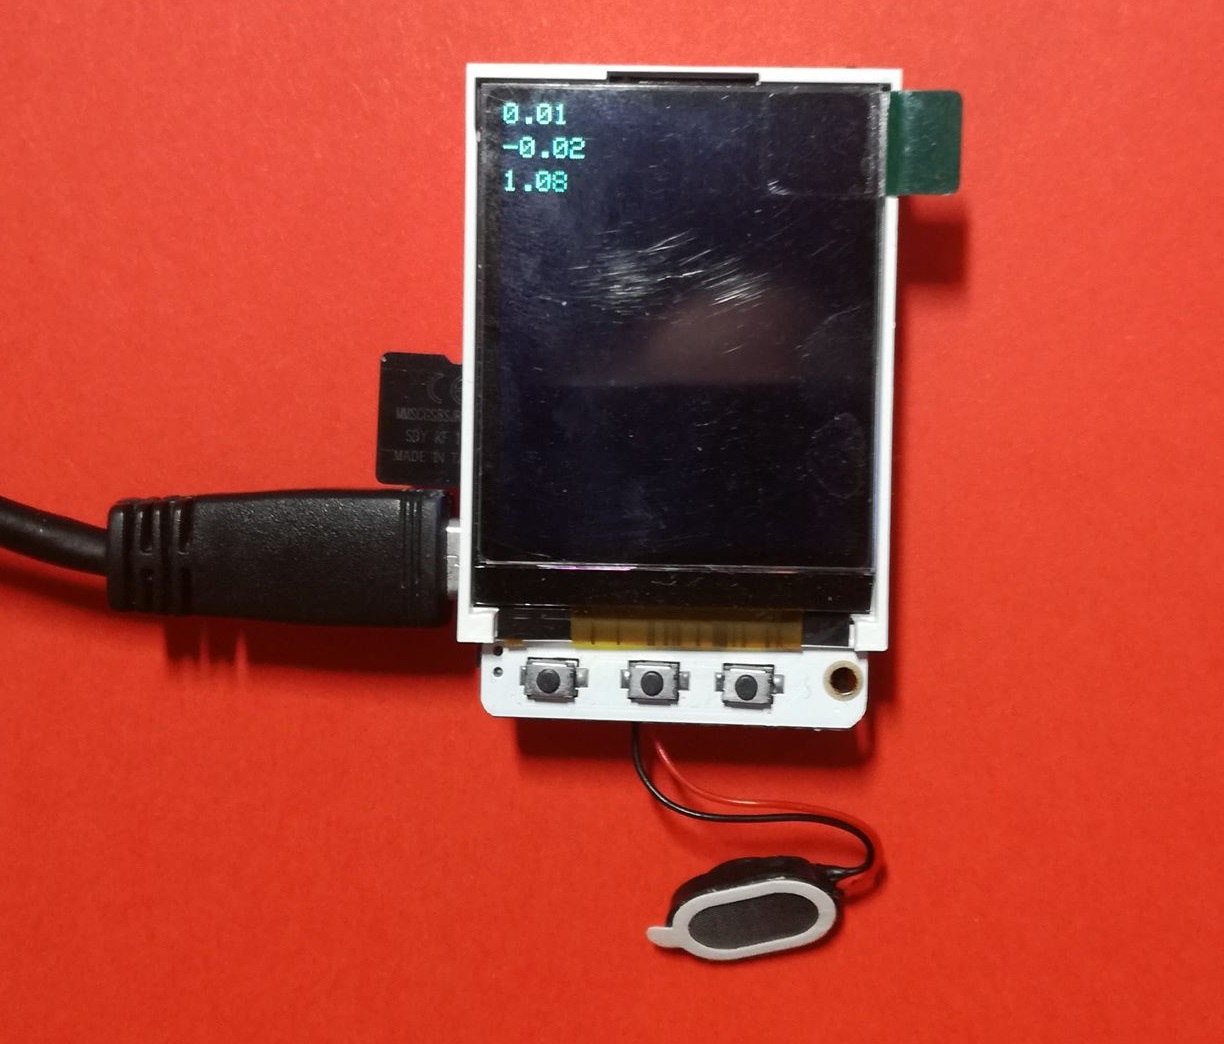
\includegraphics[width=\textwidth]{esp32_nagykijelzo.jpg}

    \subsection{Bevezetés}
      Mint azt a bevezetőben említettem, a félév első részében egy ESP32-re épülő fejlesztői lapkával foglalkoztam.
      Az ESP32 egy kedvező árú, de erős mikrokontroller-család, melyről érdemes tudni, hogy beépített Wi-Fi-vel és Bluetooth-szal rendelkezik. A szóban forgó eszköz ezen funkcionalitáson túl rendelkezik egy beépített MPU9250-el (giroszkóp, gyorsulásmérő, iránytű), SD kártya olvasóval, egy egyszerű hangszóróval és kijelzővel illetve három előlapi gombbal.

      Az eszköz programzása Arduino IDE-n keresztül lehetséges, de az ESP32 alaplapkönyvtár hozzáadása szükséges (ennek a mikéntjéről például \href{https://randomnerdtutorials.com/installing-the-esp32-board-in-arduino-ide-windows-instructions/}{itt}\footnote{Az útmutató URL-je: \url{https://randomnerdtutorials.com/installing-the-esp32-board-in-arduino-ide-windows-instructions/}} található egy leírás). Ha ez megtörtént, az \texttt{Eszközök > Alaplap} menüpontnál a felkínált lehetőségek közül válasszuk az \texttt{ESP 32 Pico Kit}-et. Így a megírt programunkat már feltölthetjük az eszközre.

    \subsection{Tapasztalatok}
      Elöljáróban szeretném megjegyezni, hogy a következőkben megemlített könyvtárak használatához szükséges egyes dolgokat beállítani az eszköz sajátosságainak figyelembevételével, ilyen beállítások a bevezetőben említett GitHub repository-ban lévő \texttt{sound2.ino}\footnote{A fájl URL-je: \url{https://github.com/awrpad/Onlab/blob/master/Arduino\%2BESP/src/sound2/sound2.ino}} fájlban találhatóak. Ebben a fájlban az itt ismertetett funkciók nagyrésze is megtalálható.

      A tapasztalatok részletesebb leírását a \textbf{kijelző}vel\footnote{A kijelzőt a használat előtt inicializálni kell, mely megtehető ezzel a kódsorral: \texttt{Adafruit\_ST7735 tft = Adafruit\_ST7735(16, 17, 23, 5, 9);}} kezdeném, hisz ez talán az eszköz legérdekesebb pontja.
      A kijelző használatához ajánlott egy már meglévő könyvtárat használni, én az Adafruit\_ST7735-öt\footnote{Adafruit\_ST7735: \url{https://github.com/adafruit/Adafruit-ST7735-Library} Az itt található fájlok közül a Adafruit\_ST7735.h fájlt ``inklúdoltam''.} használtam, ha ezt a könyvtárat az Arduino IDE-n keresztül telepítjük (\texttt{Eszközök > Könyvtárak kezelése... > \textit{\{könyvtár megkeresése a keresőben\}} > Telepítés}), automatikusan letölti az Adafruit\_GFX könyvtárat és minden egyebet, amikre ezek építenek.
      Az első dolog ami a kijelző kapcsán eszünkbe juthat, hogy szeretnénk egy egységes színt beállítani. Ezt a \texttt{fillScreen()} metódussal valósítható meg. Ez egy argumentumot vár, mégpedig a színt, amivel ki szeretnénk tölteni a képernyőt. Ehhez a feljebb említett könyvtár tartalmaz színdefiníciókat, így a teljes utasítás nézhet ki például így: \texttt{tft.fillScreen(ST7735\_BLACK);}. Itt azonban meg kell jegyezni, hogy az itt definiált színek sajnos nem feltétlenül működnek tökéletesen. A ST7735\_CYAN használatával például a sárga színnel lesz kitöltve a képernyő (de a ST7735\_BLACK például a várt módon feketével teszi ugyanezt).
      Az első képernyő átszínezés után észre fogjuk venni, hogy ez a metódus lassú. Szemre azt lehet mondani, hogy úgy egy másodperc környéki időt vesz igénybe. Nyilvánvaló, hogy ez a sebesség erősen korlátozza a modul felhasználhatóságát. Például, ha egy értéket szeretnénk rendszeresen frissítve megjeleníteni a képernyőn, a törlés és kiírás ideje könnyen lehet túlzottan lassú.
      Az ilyen és ehhez hasonló helyzetek megoldására használhatjuk például a \texttt{fillRect()} metódust, mely egy megadott téglalapot a megadott színnel kitölt. Ilyen módon nem szükséges az egész kijelzőt frissítenünk, lehetséges csupán a megadott terület egy színnel való kitöltése. Ezt kombinálva például a \texttt{tft.print("uzenet")} metódussal aránylag gyorsan is képesek vagyunk változó értékeket a képernyőn megjeleníteni. Az egyetlen problémát az így létrejövő villódzás jelenti, de az értékek még ilyen módon is könnyen leolvashatóak maradnak (amint ez látszik akkor is, ha a fent említett vázlatot futtatjuk a panelen). Természetesen az így megjelenő szöveg színe illetve mérete is befolyásolható a \texttt{tft.setTextSize(1)} illetve \texttt{tft.setTextColor(0x5FCC)} metódusokkal. Ha nem megfelelő a szöveg elhelyezése, kiiratás előtt a \texttt{tft.setCursor(0, 0)} metódussal a kurzort a képernyőn belül szabaddon bárhova elhelyezhetjük.
      A kijelzőhöz kepcsolódóan érdemes még megjegyezni, hogy annak rotációját is beállíthatjuk. Ha ezt a kódban nem tesszük meg, alapértelmezés szerint ``portré'' módba lesz az eszköz orientációja beállítva (mint egy okostelefon: alul gombok, felül a képernyő a hosszabb oldalakat bal/jobb oldalként használva). Ezt módosítani a \texttt{tft.setRotation(1)} metódussal lehet, ami például az itt használt 1-es értéket megkapva a kijelző tájkép orientációjú lesz, a gombokkal a jobb oldalon.

      A másodikként bemutatásra kerülő funkció a \textbf{hangszóró}. Ennek a használatához először is szükség van egy könytárra, melyet a következőképp használhatunk: \texttt{\#include "esp32-hal-ledc.h"} (Figyelem! Az idézőjelek használata relációs jelek helyett nem véletlen, a megfelelő alaplap kiválasztása után ez a könyvtárat így kell importálni az alkalmazásunkba).  Ha nem választottuk még ki a korábban említett alaplaptípust, akkor kaphatunk egy hibaüzenetet, mely szerint a fájl nem létezik. Ez a hiba azonban a helyes típus kiválasztásával orvosolható. Hogy megfelelően használhassuk, a setup részben be kell állítani a hangszórót, ezt az \texttt{ledcSetup} illetve \texttt{ledcAttachPin} metódusok megfelelően paraméterezett hívásával tehetjük meg. A megfelelő paraméterek a mellékelt forráskódban megtalálhatóak.
      A beállítás után a \texttt{ledcWriteTone(TONE\_PIN\_CHANNEL, 440)} metódushívással játszhatunk le hangot, első paraméterként a megfelelő (és beállításnál korábban már használt) csatornát, míg második paraméterként a lejátszani kívánt frekvenciát kell átadni Hz-ben (a példa tehát egy zenei A hangot fog lejátszani a hangszórón). A megadott hang lejátszása egészen addig folytatódik, amíg meg nem adunk egy újabb lejátszandó hangot. Ilyen módon, ha nem akarjuk tovább játszani az addigi hangot, meghívhatjuk az imént említett metódust 0 frekvenciaértéket átadva. Mivel több ilyen hang egymás utáni lejátszása nagyon repetitív forráskódot eredményezne, ráadásul úgy, hogy egy paraméter mindig fix, írtam egy egyszerű függvényt \texttt{void playTone(int freq)} szignatúrával, mely az átadott frekvenciát 200 miliszekundumig játsza le szálblokkoló módon.

      A következő funkció a beépített \textbf{MPU9250} szenzor. Amint azt a bevezetőben is említettem, ennek a szenzornak három különböző funkcionalitása van:
      \begin{itemize}
        \item Giroszkóp
        \item Gyorsulásmérő
        \item Iránytű
      \end{itemize}
      Mint eddig, most is akkor lesz a legegyszerűbb a dolgunk, ha egy könyvtárat használunk. Ehhez a szenzorhoz több könyvtárat is lehet találni, melyek közül próbáltam többet is használni, nekem a \texttt{MPU9250\_asukiaaa}\footnote{A felhasznált könyvtár és dokumentációja elérhető itt: \url{https://github.com/asukiaaa/MPU9250\_asukiaaa}} elnevezésűt sikerült működésre bírnom, a többivel különböző problémáim adódtak.
      Az MPU9250 használatához ezen kívül szükség van a \texttt{Wire.h} könyvtárra is, aminek beállítása szintúgy szükséges. Ezt a \texttt{Wire.begin(SDA\_PIN, SCL\_PIN);} kódsorral tehetjük meg\footnote{Amint az a fájlban is látható, az SDA\_PIN értéke 19, míg az SCL\_PIN konstanst 18-ra kell állítani.}. Amint ezekkel a beálításokkal elkészültünk, a szenzor könyvtárát ``össze kell kötni'' a Wire library-vel, ezt a következőképp lehet: \texttt{mpu.setWire(\&Wire);}. Továbbá szükséges még a használni kívánt funkciók inicializálása, amit a \texttt{begin...} alakú metódushívásokkal tehetünk meg. A következő kódrészlet például megteszi ezt a gyorsulásmérővel és az iránytűvel:
      \begin{lstlisting}
        mpu.beginAccel();
        mpu.beginMag();
      \end{lstlisting}
      Miután sikeresen beállítottunk mindent, a szenzort a következőképp használhatjuk: először a megfelelő \texttt{...Update} végződésű metódus hívásával frissítjük a szenzor megfelelő adatait, majd a \texttt{...<[X][Y][Z]>} alakú függvénnyel kiolvassuk a kívánt adatot.
      A következő kódrészlet például frissíti és kiolvassa a gyorsulásmérő szenzor adatait a három tengely mentén:
      \begin{lstlisting}
        // After setting up the MPU9250 and the screen
        float aX, aY, aZ;

        mpu.accelUpdate();
        aX = mpu.accelX();
        aY = mpu.accelY();
        aZ = mpu.accelZ();
      \end{lstlisting}
      Hasonló módon kell dolgozni a giroszkóppal is (\texttt{gyro}) és az iránytűvel (\texttt{mag}) is.

      Hátra van még az \textbf{SD kártya foglalat} bemutatása\footnote{Ennek a résznek a mintakódja nem a korábban említett fájlban, hanem a \url{https://github.com/awrpad/Onlab/blob/master/Arduino\%2BESP/src/espsd/espsd.ino}-ban található.}. Ahogy eddig, most is érdemes egy könyvtárat használni. A lapka dokumentációja alapján a \texttt{mySD.h} fájl használata javasolt, azonban ezt telepítenünk kell. Ráadásul sajnos nem lehetséges a szokásos módon a ``Könyvtárak kezelése'' menüpontnál importálni, hanem le kell tölteni GitHub-ról: \url{https://github.com/nhatuan84/esp32-micro-sdcard}. Itt töltsük le az egész repository-t ZIP állományként, ezután az Arduino IDE-ben: \texttt{Vázlat > Könyvtár tartalmazása... > .ZIP könyvtár hozzáadása... > \textit{{válasszuk ki a letöltött ZIP fájlt}} > Open}. Ezzel a fejlesztőkörnyezet megcsinál minden szükséges lépést és innentől kezdve a könyvtárat használhatjuk a vázlatainkhoz. Ebben az esetben is az inicializálással kell kezdeni, amelyet jelen esetben a \texttt{SD.begin(13, 15, 2, 14)}\footnote{A megadott számok ezen esetben nem példák, a felhasznált modulhoz pontosan ezek az értékek kellenek. Más eszköz használata esetén természetesen ezek változhatnak.} függvényhívással tehetünk meg. Mely tájékoztat is minket a sikerességről: ha sikerült az SD modul inicializálása, \texttt{true} értékkel tér vissza, különben \texttt{false}-al.

    \subsection{Konklúzió}
      Általánosan elmondható, hogy maga a fejlesztői eszköz hasznos és sokrétű. Különféle alkalmazásokban gyakran előforduló elemek találhatóak meg benne beépítve, ami fejlesztés során sok forrasztástól és kábelrengetegről kímélhet meg minket.
      Azonban sajnálatos a megfelelő dokumentáció hiánya, így a vele történő korai munka nehézkes lehet, plusz szerintem a GPIO pinek elhelyezése sem optimális.
      Azonban amint megismerkedtünk a lapkával a rendelkezésre álló mintakódok alapján, ha tisztában vagyunk a korlátaival, összességében egy sokrétűen és jól használható eszköz lesz a kezünkben.

  \section{Mikrofon és spektrumanalizátor}
    \subsection{Bevezetés}
      A félév során a másik nagyobb feladatom egy mikrofon modul használata volt, illetve egy, az így beolvasott hangok folyamatos elemzésére alkalmas szoftver készítése.

    \subsection{A mikrofon modul}
      Ez a modul egy egyszerű eszköz, melynek csupán három lába van, ebből egy kell a 3.3 vagy 5 Voltnak, egy a földelésnek, a maradék egy lábon pedig a beolvasott értékeket kaphatjuk meg analóg módon. Ebből fakadóan csak olyan eszközzel használható közvetlenül, melyben van beépített A/D konverter (így például egy Raspberry Pi önmagában nem elég). Viszont egy ilyen miniszámítógép teljesítményére szükségünk van az adatok feldolgozásához, ennek áthidalására természetesen használhatunk egy külső analóg-digitális átalakítót, én azonban azt a megoldást választottam, hogy az adatokat egy Arduino UNO segítségével olvastam be és onnan továbbítottam a Raspberry felé.

      Az ezen feladathoz kapcsolódó forráskódok két fájlban találhatóak meg, az Arduino-n futtatott kód a \href{https://github.com/awrpad/Onlab/blob/master/Arduino\%2BESP/src/soundComm/soundComm.ino}{\texttt{soundComm.ino}}\footnote{A soundComm fájl URL-je: \url{https://github.com/awrpad/Onlab/blob/master/Arduino\%2BESP/src/soundComm/soundComm.ino}}-ban, míg a Raspberry Pi-n lévő kód a \href{https://github.com/awrpad/Onlab/blob/master/RPi/src/spectrum\_analyzer.py}{\texttt{spectrum\_analyzer.py}}\footnote{A spectrum\_analyzer fájl URL-je: \url{https://github.com/awrpad/Onlab/blob/master/RPi/src/spectrum\_analyzer.py}} fájlban.

    \subsection{Adatok beolvasása}
      Amint az előző részben említettem, a mikrofon adatait analóg módon lehet beolvasni például egy Arduino lapkával. Mivel az adatokat egyesével átküldeni eléggé pazarló és lassú lenne, így azt a megoldást választottuk, hogy először magán az Arduinon beolvasunk és eltárolunk valamennyi adatot, majd ezeket egy csomagként küldjük át a Raspberry-re. Végül az 500 darab beolvasott érték / csomag méretet választottam, mert ez még kényelmesen elfért az Arduino UNO memóriájában (míg például 1000 darab már nem fért volna be). Egy ötlet lehetne, hogy az \texttt{int} típus helyett \texttt{short} típust használjunk, azonban ezen az Arduino típuson ez nem jelentene különbséget \footnote{Vesd össze: \url{https://www.arduino.cc/reference/en/language/variables/data-types/int/} és \url{https://www.arduino.cc/reference/en/language/variables/data-types/short/}}. Azonban az ennél kisebb, egy bájtos típus mérete pedig nem lenne elég, hiszen az \texttt{analogRead()} függvény által visszaadott értékek 10 bitesek.

      Ehhez kapcsolódóan azonban előkerül egy korlátozás is. Mivel az olvasáshoz az előbb említett függvényt kell használni, egyértelmű, hogy annak a sebessége korlátoz. Talán nem is gondolunk bele, de ez hang esetén például valós korlátozás lehet, ugyanis egy \texttt{analogRead()} hívás nagyjából 0.1 miliszekundumig tart, ami azt jelenti, hogy a maximális mintavételi rátánk 10000/s\footnote{Arduino dokumentáció - analogRead(): \url{https://www.arduino.cc/reference/en/language/functions/analog-io/analogread/}}, ebből adódóan lefgeljebb nagyjából 5000 Hz-es hangokat tudunk megfigyelni (ami az emberi beszédet elég jól lefedi, de amennyiben ezt diagnosztikai eszközként szeretnénk használni, akkor kevés lehet).

    \subsection{Kommunikáció}
      Természtesen az Arduino-n beolvasott adatokat valamilyen módon továbbítani kell a Raspberry-re. Adja magát a módszer, hogy a két eszközt USB-n keresztül kössük össze, úgyhogy én is ezt tettem\footnote{Szerencsére USB-s összekötés esetén nem kell foglalkoznunk a lapkák jelszintkülönbségével.}.

      Több próbálkozás és helytelen módon működő kommunikáció után arra jutottam, hogy az eszközök kommunikációjához mindenképpen szükség lesz egyfajta protokollra. Ebben a protokollban meghatároztam a küldött csomag felépítését és a küldés módját. A küldött csomag a következőképp épül fel:
      \begin{itemize}
        \item -1 : Egy fix érték, ami a csomag elejét jelzi
        \item Az 500 beolvasott adat (időben a legelső beolvasottal legelől)
        \item Az adatok beolvasására felhasznált idő miliszekundumban
        \item -3 : Egy újab fix érték, ami a csomag végét jelzi.
      \end{itemize}
      A küldés módjában a következőket határoztam meg: Az adatok továbbítása USB-n történik (Arduino-ban \texttt{Serial.println()}). A fogadónak jeleznie kell, ha készen áll az adatok fogadására \footnote{Ilyen szempontból szerencsés, hogy a Raspberry Pi által használt logikai magas értéket (3.3V) az Arduino is igaz értéknek érzékeli, így a különböző jelszintek itt nem korlátoznak.}. Ezt az Arduino egy előre meghatározott pin-jére írt logikai magas értékkel teheti meg. Adatok akkor és csak akkor lesznek küldve, ha a fogadási szándékot jelezték.
      Ezen szabályok betartásával biztosítható lett, hogy az adatok egyértelműen kiolvashatók legyenek és hogy azok a lehető leghamarabb rendelkezésre álljanak a küldéshez. Amíg ez a protokoll nem létezett, lehetséges volt, hogy például egy tömb közepén kezdjen el olvasni a Raspberry, ami nem megengedhető, hiszen szükséges átküldeni a beolvasás időhosszát is. De az is előfordult, hogy az Arduino olyan adatok átküldésével foglalkozott, amiket végül nem is használt fel a Raspberry-n futó program, így feleslegesen töltött el időt a lassú adattranszferrel, ahelyett, hogy a gyors beolvasással foglalkozott volna. Így a ténylegesen felhasznált adatok késleltetése nőtt.

      A használt mérési elrendezés az alábbi ábrán látható: 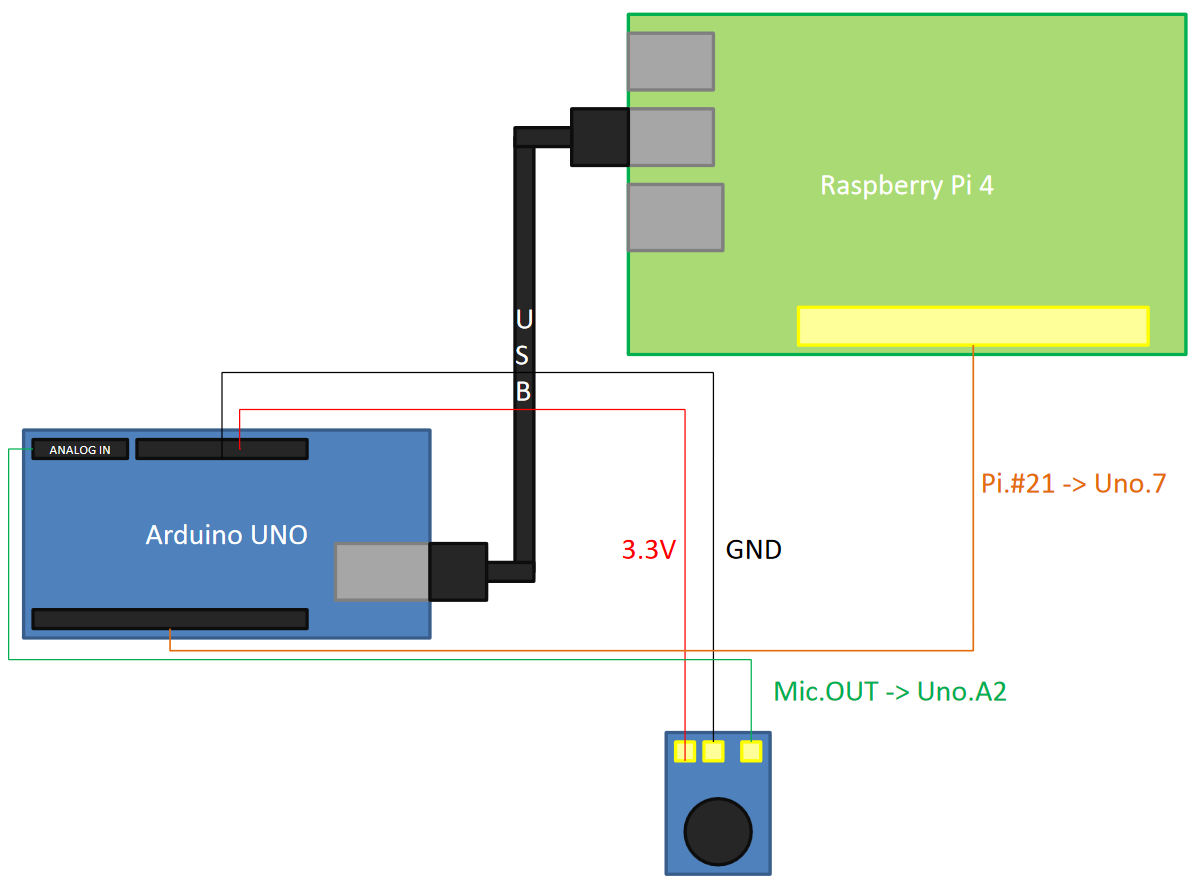
\includegraphics[width=\textwidth]{elrendezes.png}


      A két eszköz kommunikációja ebben a megvalósításban bár biztos és aránylag hatékony, azért lehetne még rajta fejleszteni. Az USB-n keresztül történő kommunikáció \texttt{Serial.println()} használatával például nagyon pazarló. Ilyen módon ugyanis sztringként történik az adatátvitel, tehát a számokat előbb át kell alakítani ilyen adattípussá, majd vissza számmá, ez nagy overhead-et jelenthet. Természetesen a baud rate emelésével gyorsíthatjuk a kommunikációt, de érdemes lehetne például kipróbálni, hogy milyen sebességnövekedést tudunk elérni, ha az Arduino és a Raspberry lábait kötjük össze. \textbf{Figyelem!} Ha ezt a megoldást használjuk, elővigyázatosnak kell lennünk, ugyanis az Arduino UNO és a Raspberry Pi más jelszinten működik (5V illetve 3.3V), ilyen módon a közvetlen összeköttetés tönkre teheti a Raspberry-t, mivel az van kisebb feszültségre tervezve (és nem mellesleg ez nagyságrendekkel drágább is). Erre megoldást jelenthet az UNO helyett egy másik eszköz használata (például valamelyik ESP, hiszen azok is 3.3 Volttal működnek, de vannak már ilyen jelszintű Arduino-k is), vagy használhatunk egy jelszintillesztő áramkört is.

    \subsection{A spektrumanalizátor alkalmazás}
      A sikeresen beolvasott és átküldött adatokat fel is kell valahogy dolgozni. Ennek érdekében egy Raspberry Pi-n futó spektrumanalizátor alkalmazást\footnote{Az elkészült alkalmazás a \url{https://github.com/awrpad/Onlab/blob/master/RPi/src/spectrum_analyzer.py} helyen elérhető.} készítettem. Mivel ehhez sok összetett műveletet kell elvégezni, jó lett volna, ha ezekhez (például FFT, grafikonrajzolás) már meglévő eszközöket tudok használni. Elsősorban ez indokolta a döntést, hogy Python nyelven valósítsam meg ezt a programot (továbbá ezen a nyelven könnyen kezelhetők a Raspberry Pi GPIO lábai, illetve az USB).

      Szeretnénk tehát látni, hogy a mikrofon által érzékelt hang hogyan épül fel. Ehhez a beolvasott jelet természetesen Fourier-transzformációnak kell alávetni. Mivel szeretnénk valós időben végezni a vizsgálatot (vagy ahhoz a lehető legközelebb), természetesen az Fast Fourier Transformation-t (FFT) érdemes alkalmazni. Szerencsére Python nyelvben léteznek már kész kódkönyvtárak erre. Az én választásom ezek közül is a \texttt{scipy.fftpack.fft()}-re esett. Ez a könyvtár kifejezetten népszerű és jól dokumentált. Ezen szempontok kezdő ``pythonosként'' közel a könnyű használhatósággal megegyező fontosságú szempontok (szerencsére ilyen szempontból is jól teljesít).
      Fontos megjegyezni, hogy az ilyen módon előállított értékek mértékegysége nem Hz. Hogy le tudjuk olvasni a frekvenciákat, a grafikon vízszintes tengelyét külön skálázni szükséges.

      Az következő fontos alkalmazáskomponens a grafikonrajzoló modul. Első próbálkozásként a \textbf{Matplotlib} könyvtárat használtam, hisz ez tűnt a legnépszerűbbnek. Ennek a könyvtárnak a használata egyszerű, az egész könnyen beállítható és ha valahol elakadunk, az interneten szinte biztosan kapunk választ a kérdésünkre. Azonban használat közben észre kellett vennem, hogy nem ez a legmegfelelőbb könyvtár ehhez az alkalmazáshoz. A Matplotlib ugyanis elsősorban arra koncentrál, hogy a létrejövő grafikonok olyan minőségűek legyenek, hogy azokat akár egy publikációban is meg lehessen jeleníteni. Ez természetesen önmagában még nem baj, azonban a szépség ebben az esetben a sebesség rovására is megy. Ezért indokolt volt keresni egy olyan könyvtárat, mely a sebességet részesíti előnyben. Így találtam rá a \textbf{PyQtGraph}-ra\footnote{Matplotlib: \url{https://matplotlib.org/}, PyQtGraph: \url{http://www.pyqtgraph.org/}}. Szerintem az alap beállításokat valamivel nehezebb volt elvégezni, azonban a megjelenítés szemmel láthatóan gyorsabb lett. Továbbá a felmerülő kérdéseinkre bár kaphatunk választ interneten keresztül, de leginkább a mellékelt példákból\footnote{A PyQtGraph-hoz mellékelt példakódok futtatásának leírása: \url{https://pyqtgraph.readthedocs.io/en/latest/introduction.html\#examples}} tanulhatunk.

      A következő lépés a kiugró értékek megkeresése a kapott jelben. Szerencsére mivel Python-t használunk, természetesen erre is van már készen implementált algoritmus. Ez pedig a \texttt{scipy.signal} könyvtárban található \texttt{find\_peaks()} függvény, melynek egy kötelezően megadandó paramétere van, mégpedig maga a jel, amit fel kell dolgoznia. Azonban ha csak így használjuk, minden ilyen értéket megtalál, a nagyon aprókat is. Hogy ezt a működést felülírjuk, több opcionális paramétert is megadhatunk. Hogy ezek pontosan mik és mit jelentenek, annak a dokumentációban\footnote{\texttt{find\_peaks()} dokumentáció: \url{https://docs.scipy.org/doc/scipy/reference/generated/scipy.signal.find\_peaks.html}} érdemes utánanézni. A függvény visszatérési értéke egy tömb, melyben indexek vannak. Ezeken az indexeken találhatóak az átadott tömbben a kiugró értékek. \textbf{Megjegyzés}: ezt a funkciót a program egy korábbi verziójában (még Matplotlib-bel) használtam, azonban a jelenlegi verzióban még nincs benne a használata, csupán egy kikommentezett kódsor, mely finomhangolásra szorul. Ezt a következő módon tettem meg:
        \texttt{fft\_x\_axis = np.linspace(0.0, 1.0 / (2.0 * avg\_sample\_duration), N/2)}
      Ezek után a dolgunk az, hogy a \texttt{plot()} metódus első paramétereként az imént létrehozott \texttt{fft\_x\_axis} változót adjuk át, második paraméterként pedig az FFT által visszaadott értékek kellenek, megfelelően átdolgozva. Ezt az árdolgozást a következőképpen tehetjük meg: \texttt{fft\_to\_plot = 2.0 / N * np.abs(fft\_values[:N//2])}
      Ahol N a beolvasott adatok száma.

      Az elkészült programot a következőképp használhatjuk (feltételezve, hogy a méréshez szükséges dolgoket megfelelően összeszereltük): Futtassuk a \texttt{spectrum\_analyzer.py} fájlt (például egy fejleszőkörnyezetből). Ezután rögtön látni fogjuk a bejövő adatokat: a felső diagramon a nyers beolvasott adatok láthatók, míg alul a feldolgozottak. Ha az alső diagram fölé visszük az egér mutatóját, az ábra felett bal oldalt leolvasható az X tengely értéke, így leolvasható az adott frekvencia (MHz-ben).

    \subsection{Mérések a spektrumanalizátorral}
      Az elkészült programot természetesen ki is próbáltam. Ehhez a telefonomra letöltöttem egy appot, mely képes megadott frekvenciájú hangok lejátszására. Az itt bemutatott mérések során a beállított frekvencia mindig 440 Hz volt.

      Az első lejátszott hang \textbf{szinuszos} formájú volt. A programban ez az alábbi módon jelent meg:
      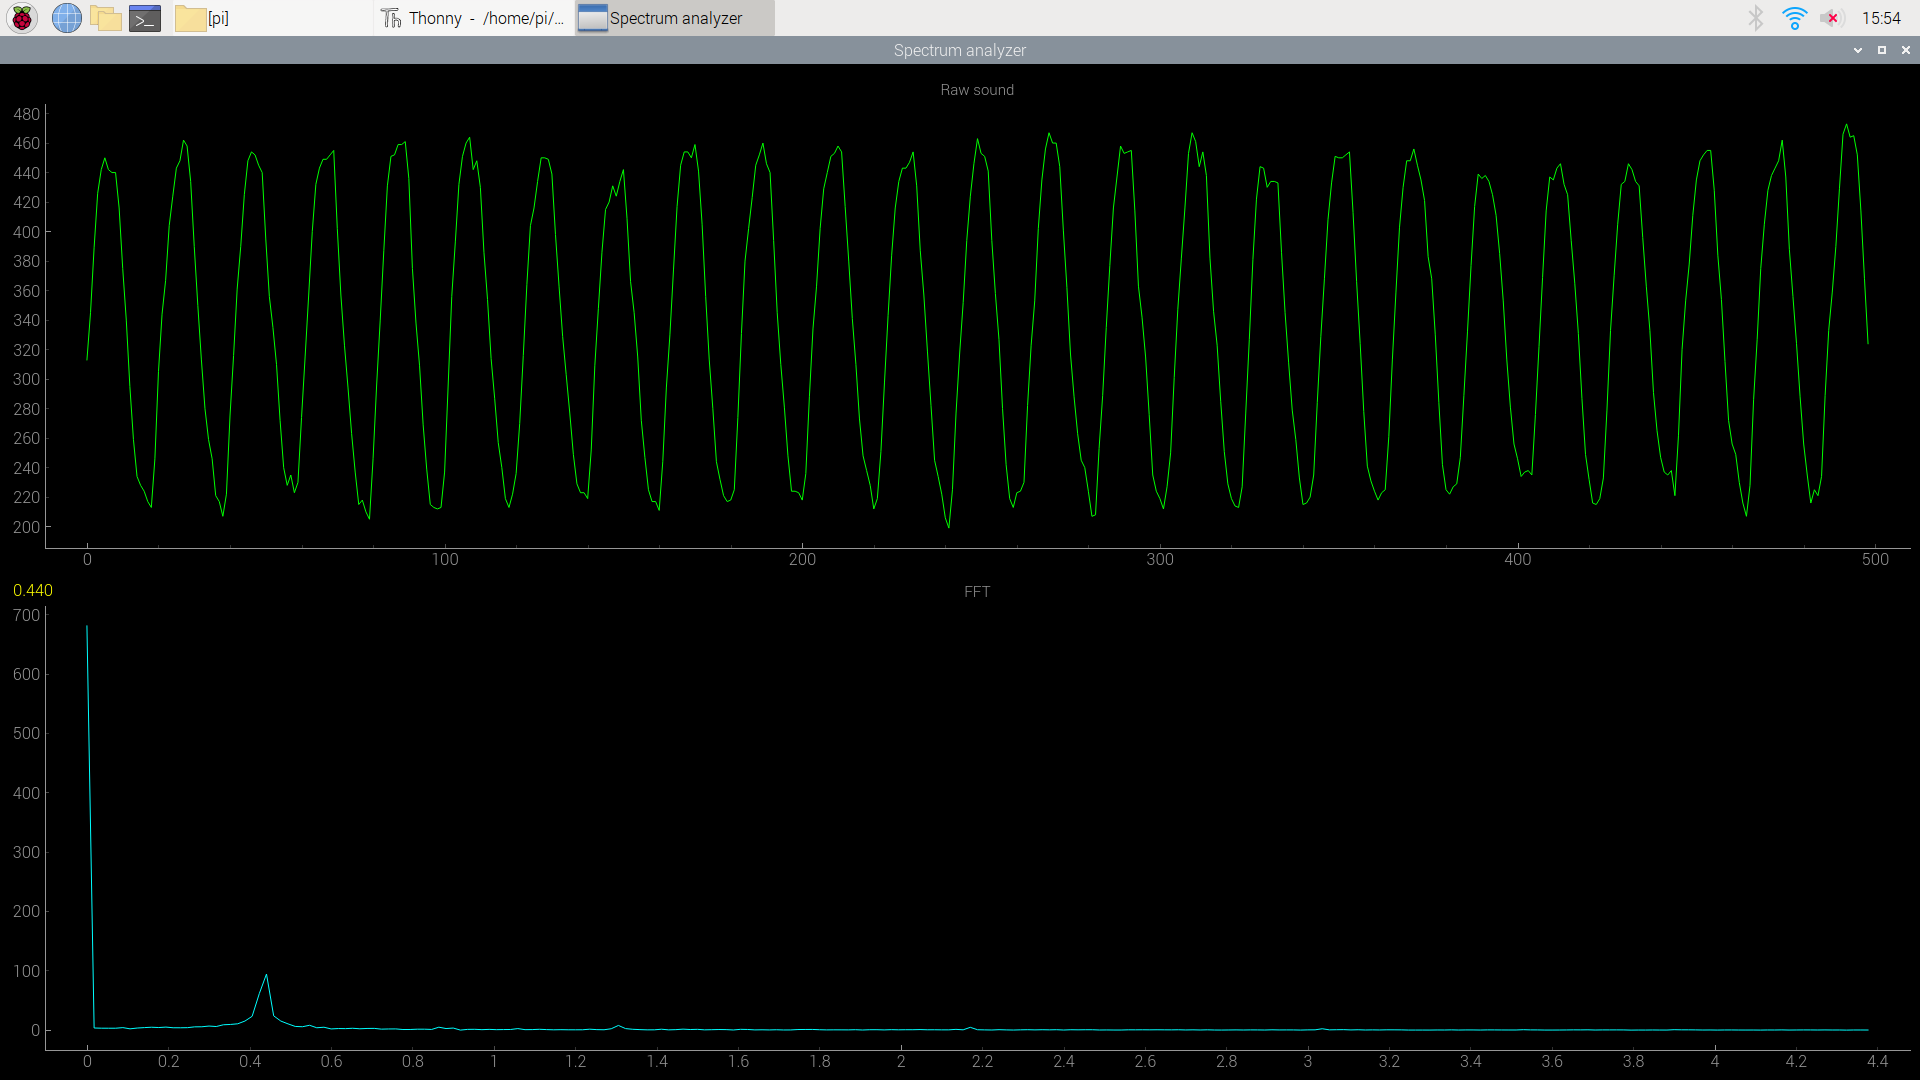
\includegraphics[width=\textwidth]{s_a_sin.png}
      A felső grafikonon látszik, hogy a vett jel nem lesz tökéletes szinusz, de megközelítőleg jó. Ez lehet a telefon hangszórójának hibája, illetve a mikrofon hibája is (de legvalószínűbb, hogy mindkettő). A jel formája valamennyivel javul, ha a telefon a mikrofonhoz képest optimálisabb helyzetben van. Bár a képernyőképen nem látszik, az egérmutató az alsó grafikon első kiugró érétkének csúcsánál van. Emiatt le is olvasható a 0.440 érték baloldalt, amiből látszik, hogy a hang 440 Hz-es. Bár aránylag kicsik, de látszódnak még kisebb kiugrások, ez valószínűleg a jel tökéletlenségéből adódik.
      A következő jel egy \textbf{négyszögjel}.
      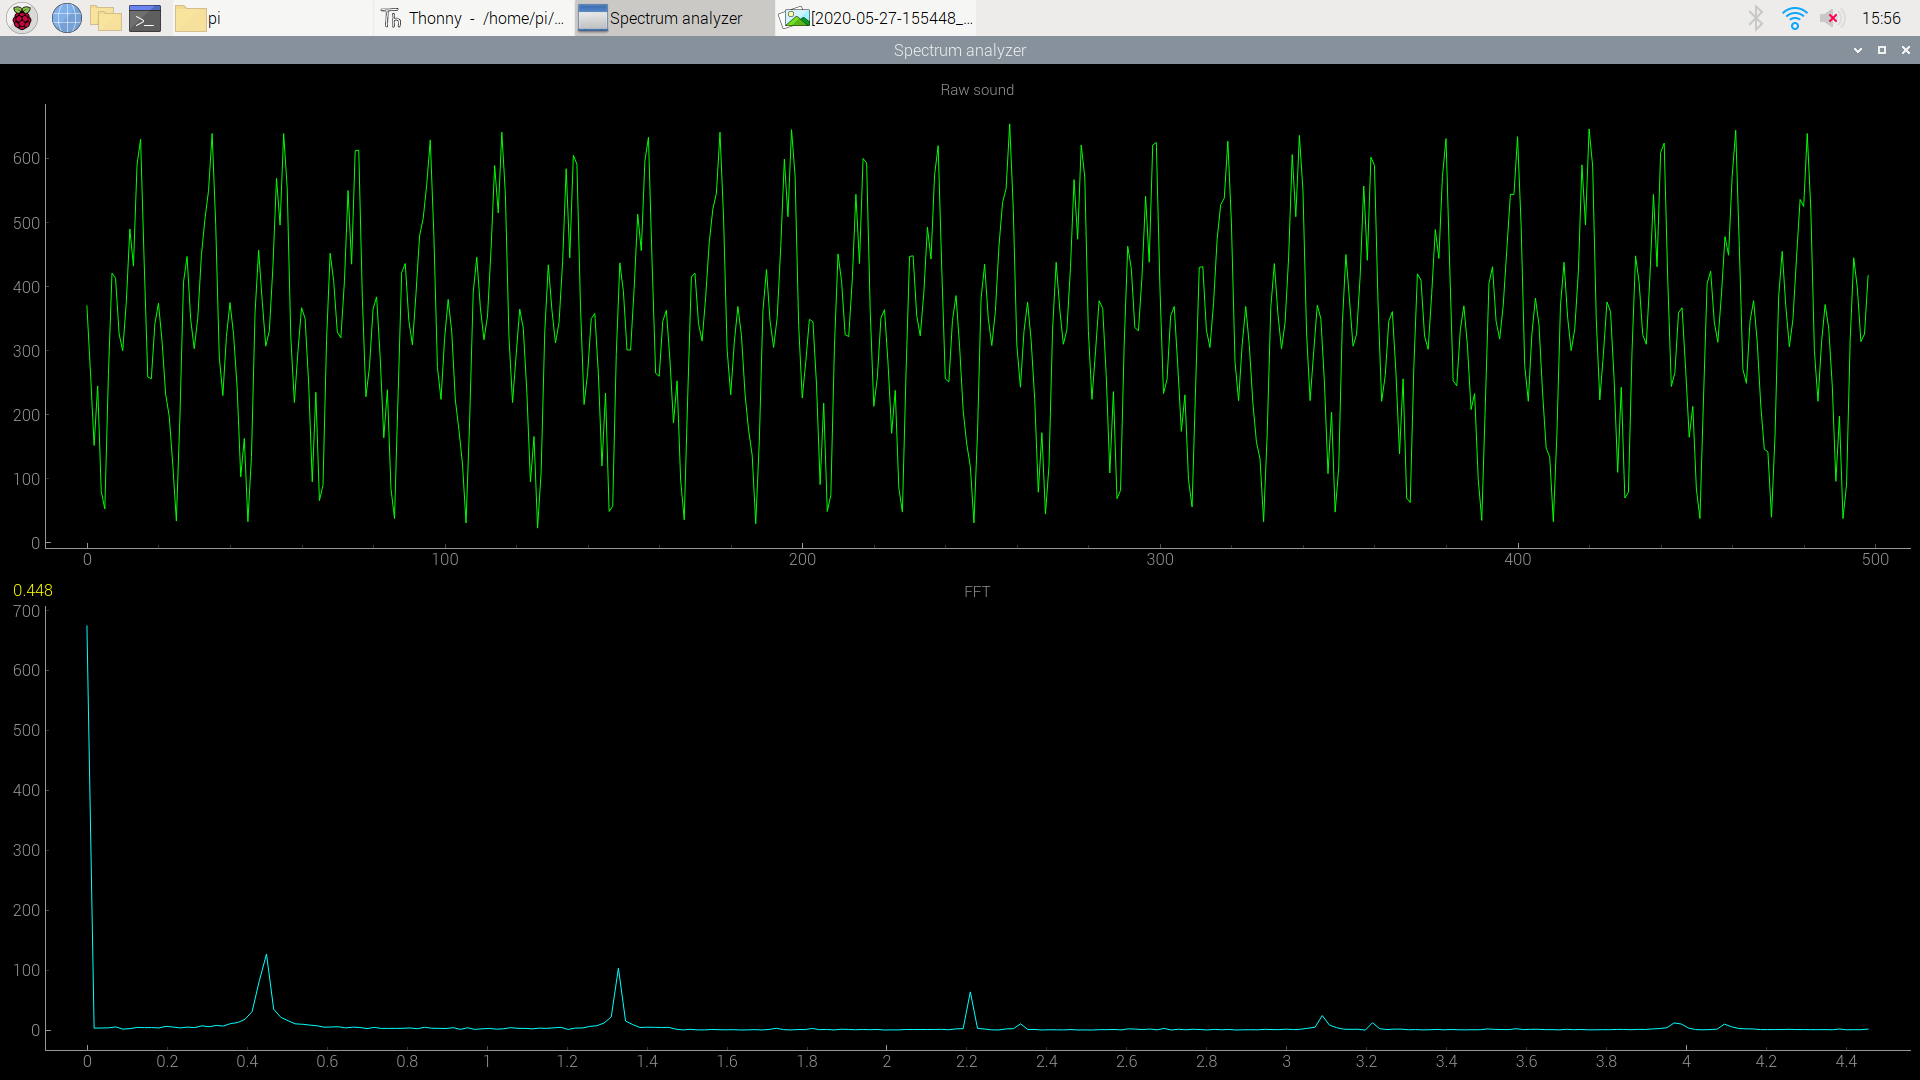
\includegraphics[width=\textwidth]{s_a_square.png}
      Sajnos elég erős absztrakciós képességekkel kell rendelkeznünk ahhoz, hogy megállapítsuk a nyers jelformáról, hogy ez négyszögjel, de szerencsére így is jól látjuk az egész program működésének lényege: a feldolgozott jelen szépen látszódnak a hang komponensei.
      Ugyanez mondható el nagyjából a harmadik mérésről is, ahol egy \textbf{fűzészfogjel} alakú hangot játszottam le.
      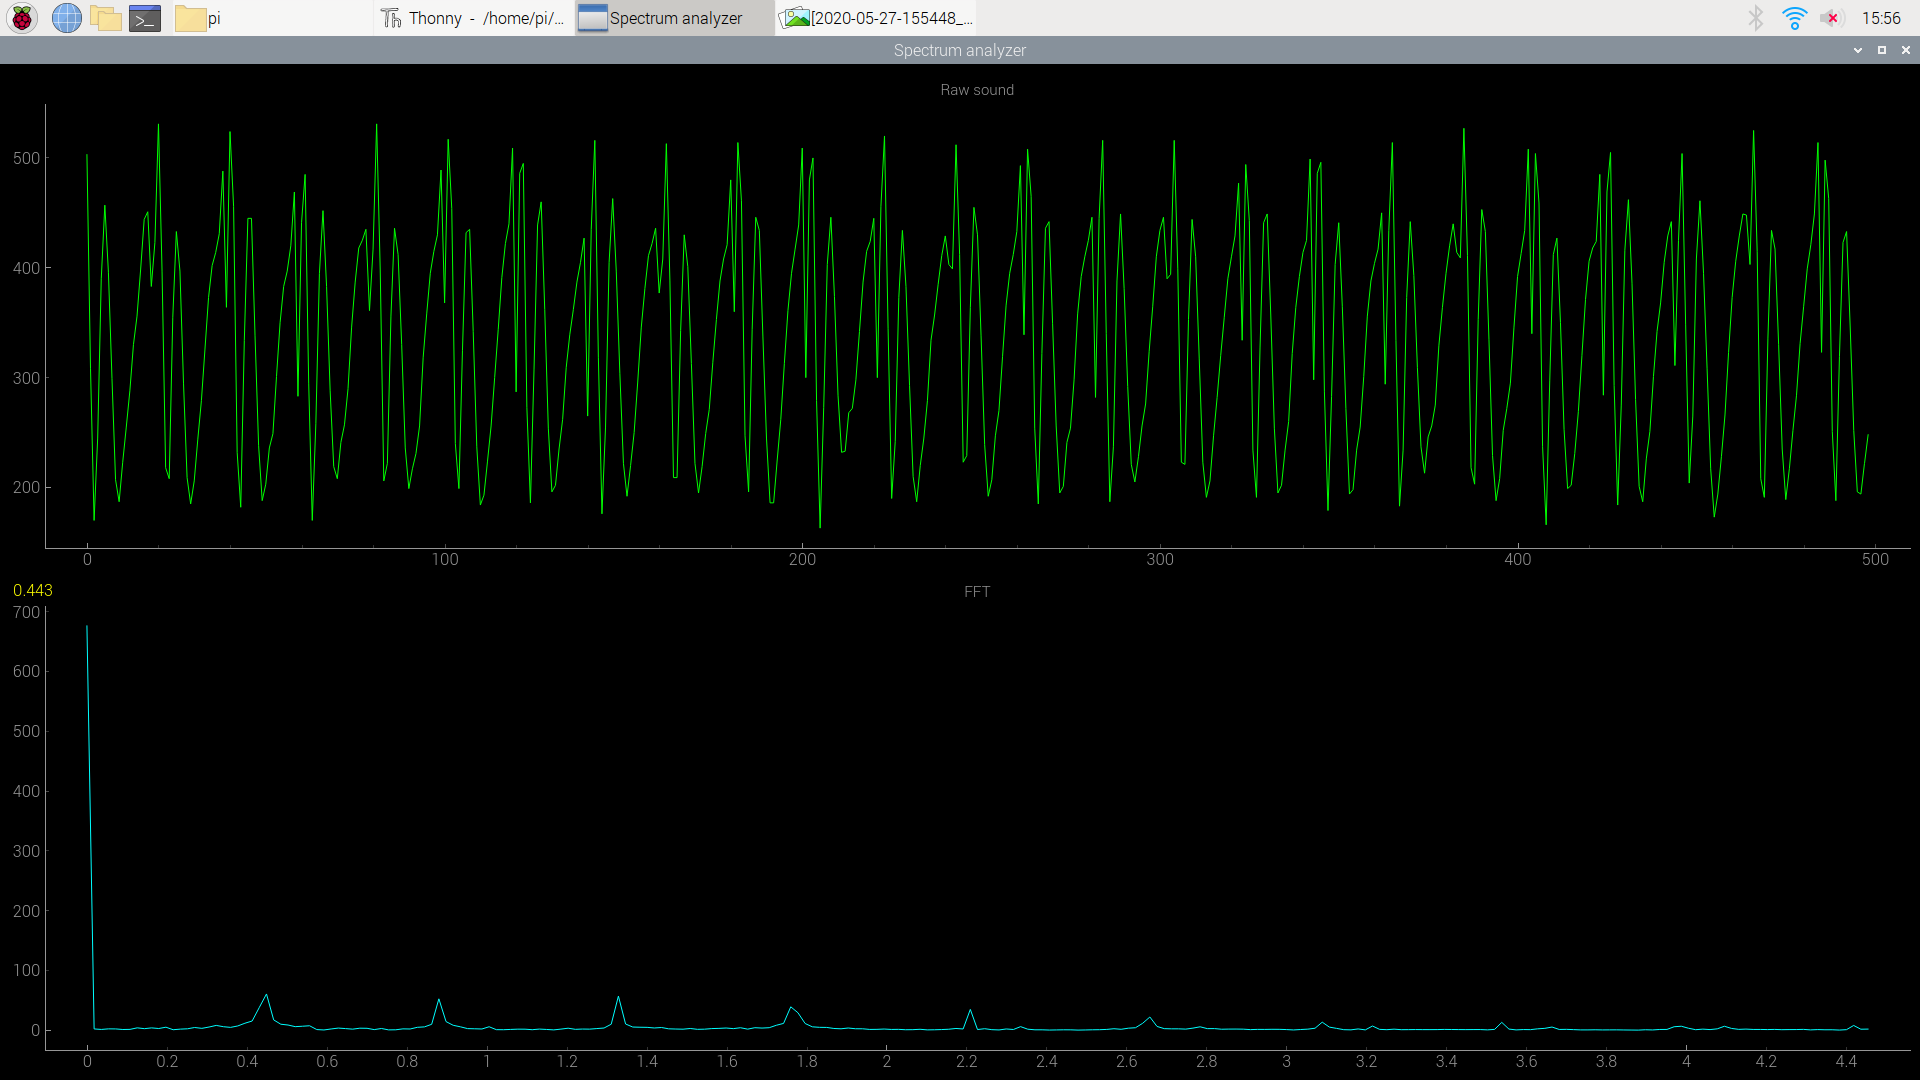
\includegraphics[width=\textwidth]{s_a_sawtooth.png}
      A nyers jel itt sem mondható szépnek, de a komponensek jól látszódnak.

      A mérések alapján azt mondhatjuk, hogy a program aránylag jól használható, egy probléma azonban adódik: Raspberry Pi-n futtatva sajnos nem a leggyorsabb, így a valósidejűségről le kell mondanunk. Épp ezért a fejlesztés következő lépése lehet megvizsgálni, hogy hogyan tudjuk gyorsítani a már meglévő alkalmazást. Ezen kívül feltűnhet még, hogy minden vizsgált jelnél van egy magas kiugrás a 0 Hz-es frekvenciánál. Erre egy megoldás lehet, ami az alábbi linken olvasható: \url{https://www.mathworks.com/matlabcentral/answers/42325-fft-is-finding-a-max-amplitude-at-0-hz}. Természetesen ez is további utánajárást igényelhet, de nem akartam ``nemes egyszerűséggel'' levágni a nullás kiugró értéket.

\end{document}
